\documentclass{article}

\usepackage{graphicx}
\usepackage{subcaption}
\usepackage[landscape]{geometry}
\geometry{total={10in,8in},left=0.25in, top=0.1in}

\begin{document}

\begin{figure}[h!]
\centering
\begin{subfigure}[b]{0.3\linewidth}
  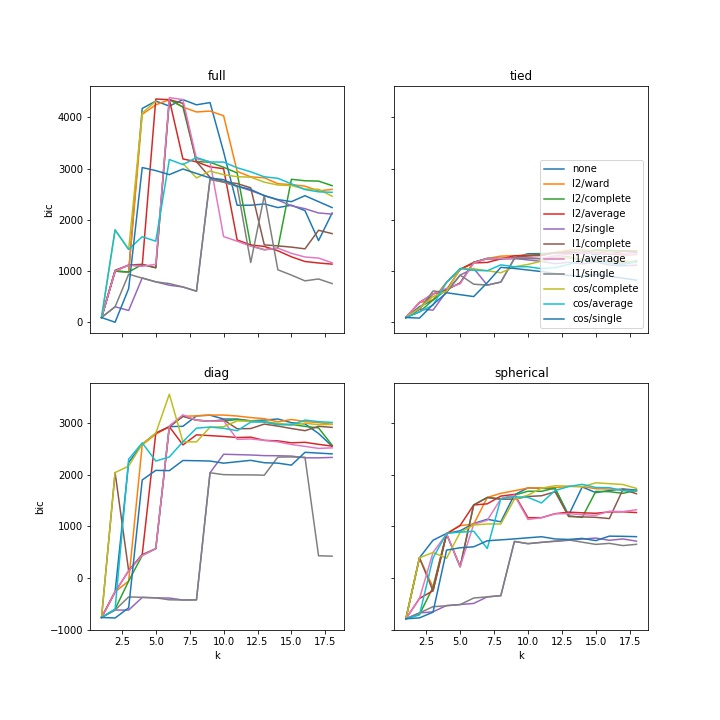
\includegraphics[width=\linewidth]{python_drosophila_bicplot.jpg}
\end{subfigure}
\begin{subfigure}[b]{0.3\linewidth}
  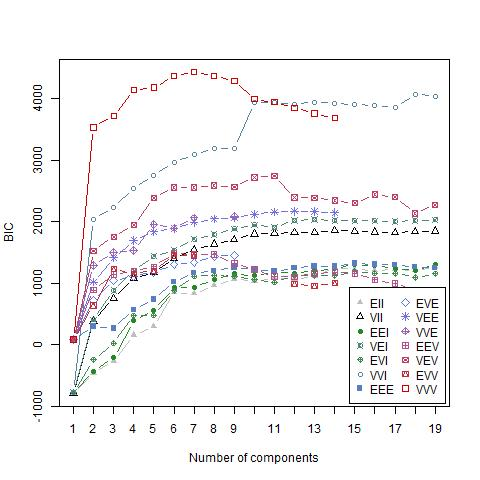
\includegraphics[width=\linewidth]{r_drosophila_bicplot.jpg}
\end{subfigure} 

\begin{subfigure}[b]{0.3\linewidth}
  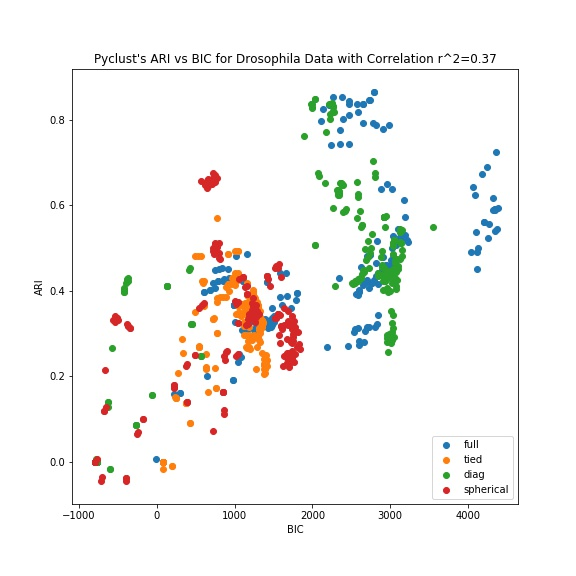
\includegraphics[width=\linewidth]{python_drosophila_bicari.jpg}
\end{subfigure}
\begin{subfigure}[b]{0.3\linewidth}
  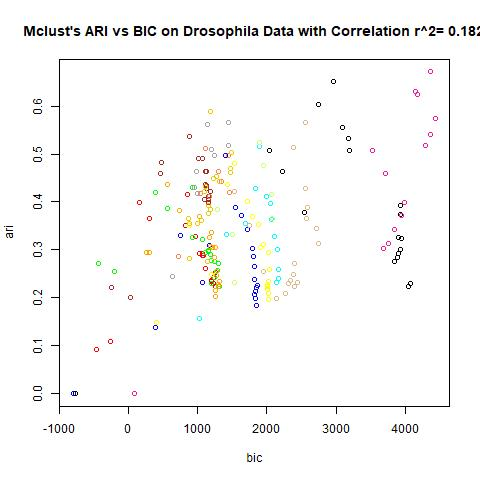
\includegraphics[width=\linewidth]{r_drosophila_bicari.jpg}
\end{subfigure} 
\end{figure}
\noindent Drosophila Data \\
The left column is using Python's clustering methods - "pyclust,"\\
The right column is using mclust. \\ \\

\noindent The top row shows the BIC results for all combinations of clustering technigues. \\
The bottom row shows the relationship between BIC and ARI for all the clustering techniques.


\newpage

\begin{figure}[h!]
\centering
\begin{subfigure}[b]{0.3\linewidth}
  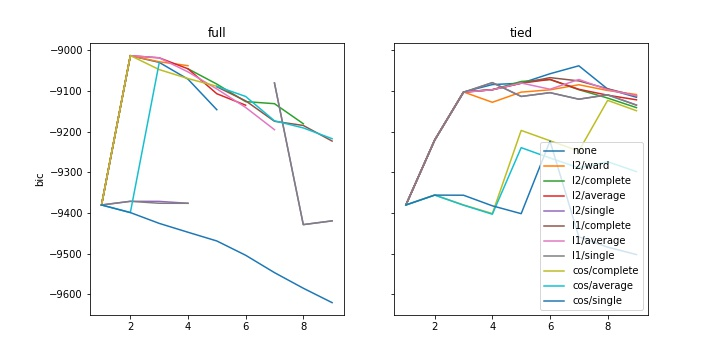
\includegraphics[width=\linewidth]{python_bc_bicplot.jpg}
\end{subfigure}
\begin{subfigure}[b]{0.3\linewidth}
  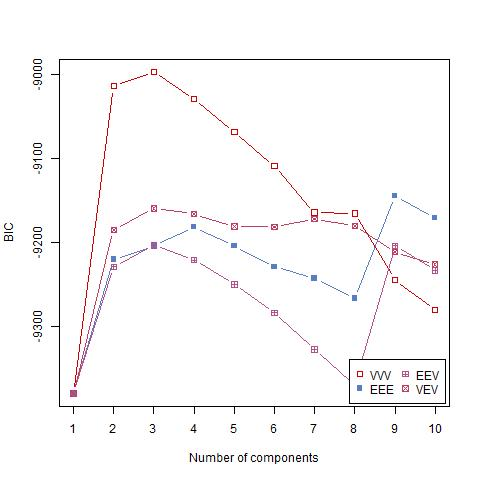
\includegraphics[width=\linewidth]{r_bc_bicplot.jpg}
\end{subfigure} 

\begin{subfigure}[b]{0.3\linewidth}
  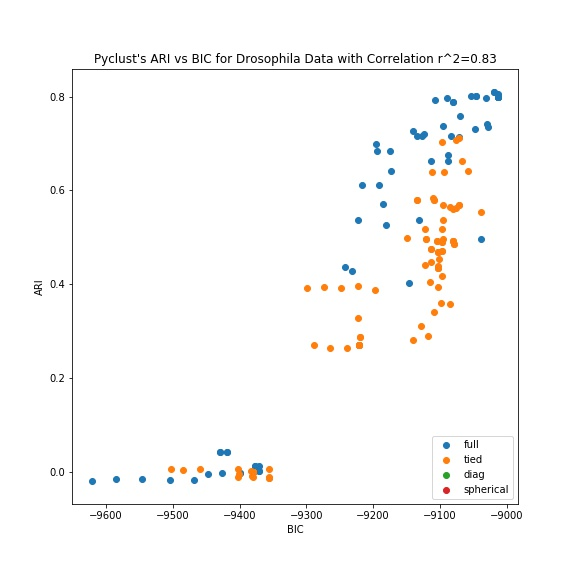
\includegraphics[width=\linewidth]{python_bc_bicari.jpg}
\end{subfigure}
\begin{subfigure}[b]{0.3\linewidth}
  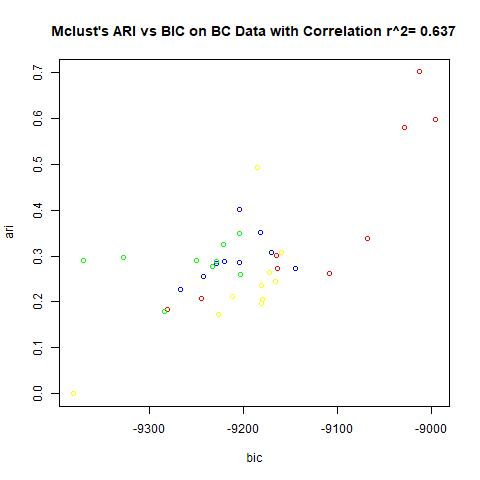
\includegraphics[width=\linewidth]{r_bc_bicari.jpg}
\end{subfigure} 
\end{figure}

\noindent Wisconsin Breast Diagnostics Dataset (http://archive.ics.uci.edu/ml/machine-learning-databases/breast-cancer-wisconsin/) \\
As you can see, I limited the number of clustering combinations for both mclust and pyclust to replicate what was done in the original paper: Fraley & Raftery. Model-Based Clustering, Discriminant Analysis, and Density Estimation.

\end{document}